% Created 2021-04-18 Sun 16:20
% Intended LaTeX compiler: pdflatex
\documentclass[11pt]{article}
\usepackage[utf8]{inputenc}
\usepackage[T1]{fontenc}
\usepackage{graphicx}
\usepackage{grffile}
\usepackage{longtable}
\usepackage{wrapfig}
\usepackage{rotating}
\usepackage[normalem]{ulem}
\usepackage{amsmath}
\usepackage{textcomp}
\usepackage{amssymb}
\usepackage{capt-of}
\usepackage{hyperref}
\date{\today}
\title{Final Reserach Report P363 (Group 3)}
\hypersetup{
 pdfauthor={},
 pdftitle={Final Reserach Report P363 (Group 3)},
 pdfkeywords={},
 pdfsubject={},
 pdfcreator={Emacs 26.3 (Org mode 9.1.9)}, 
 pdflang={English}}
\begin{document}

\maketitle
\tableofcontents



\section{Introduction}
\label{sec:orge23f03d}

The use of experimental tests have been employed in Psychology ever since it was born. Ever since then there have been the development of a number of psychological tests to measure certain variables. One particular test that has been developed uses implicit attitudes to measure a person's underlying automatic evalutation on a certain subject, this is known as the Implicit Association Test (IAT) \cite{greenwald_mcghee_schwartz_1998}. This test works by displaying target words or images on screen and having participants respond to pairs of attitude objects (e.g. self vs other) or affective concepts (e.g. positive vs negative) by pressing a left versus right response key. The reaction time to attribute the response to the target object is then taken as an indicator of implicit attitudes. Past researchers have used this method to test a variety of implicit attitudes, such as attitudes towards one parent \cite{Yang_2013} or the subjective well-being of oneself \cite{Walker_Schimmack_2008}. More notably IAT measures are often used as self-esteem measures using words to describe a person's chracteristic and measuring how fast one responds to characteristics that they might attribute to themself. Taking inspiration from the study done by Karpinski (2004) we will adopt a similar format using a word bank of describing characterisitcs to measure implicit attitudes towards self-esteem. 

\section{Method}
\label{sec:org302da94}

\textbf{Subjects}

Students from group 3 of Computing and Psychological Research course at University of Waterloo and their respective family members and friends participated in the study. The study consists of 8 subjects in total. 

\textbf{Procedure}

In the IAT, the subject responds to a series of items that are to be classified in 2 categories, one assessing the associations of self versus other and the other representing an attribute discrimination such as pleasant versus unpleasant words. The experiment consisted of 5 blocks of categorization trials. In each step, the subject presses a left or right key to categorize each stimuli which are presented on the desktop screen. The computer recorded the elapsed time between beginning of presentation of each stimulus and occurrence of keyboard response of block 3 and block 5.

Part 1 consists of instructions for the subject to understand what is needed from them. In the first step, the subjects practice a target concept by classifying items into self and other categories. The second step includes categorizing pleasant and unpleasant words. In the third step, the subject groups items into 2 integrated categories, ie, it includes the target and attribute concept, assigned to same key in the previous two steps. For instance, self+pleasant (left key), other+unpleasant(right key). The fourth step is the practice test with reverse keys for either the target or attribute concept. The last step involves switched key experiment. For example, self+unpleasant (left key) or other+pleasant(right key). 

\section{Results}
\label{sec:orgca9b8cc}

\#\#Setup for data export
\textbf{Data Structure}
Below is an excerpt sample from one of our trial experiment result CSV files. As shown below, the data collected includes the run number (exclusively from the 3rd and 5th experiment sessions), the word presented on screen, the key the participant pressed, and their respective reaction time. In addition, the average and sum of participants positive and negative word reaction times and number of correct keystrokes were calculated for each of the comparative trial sessions.

\begin{verbatim}
##Shows Data Structure Sample
head(dg, 5)
\end{verbatim}

\begin{verbatim}
  Run.Number  Word Key Reaction.Time
1          5 OTHER   p     3.6031035
2          5  SELF   q     0.5321590
3          5  SELF   q     0.9458877
4          5 ALONE   p     1.4066698
5          5  SELF   q     0.6486051
\end{verbatim}


\textbf{Table 1}
Descriptives of Reaction Times 
\#Not sure if we need a table for this or to include it, but I figured I'd put it in anyways as SDs are not included in the previous summary table

\begin{verbatim}
table_desc <- matrix(c(mean(IAT_data$Positive.Word.Reaction.Time.Average),sd(IAT_data$Positive.Word.Reaction.Time.Average),median(IAT_data$Positive.Word.Reaction.Time.Average),mean(IAT_data$Negative.Word.Reaction.Time.Average),sd(IAT_data$Negative.Word.Reaction.Time.Average), mean(IAT_data$Negative.Word.Reaction.Time.Average)), ncol = 3, byrow = TRUE)

colnames(table_desc) <- c("Mean", "SD", "Median")
rownames(table_desc) <- c("Positive Words", "Negative Words")      

table_desc <- as.table(table_desc)

table_desc
\end{verbatim}

\begin{verbatim}
                    Mean        SD    Median
Positive Words 0.8545347 0.3109061 0.7911803
Negative Words 0.9436601 0.3209012 0.9436601
\end{verbatim}





\textbf{T-Tests}
\begin{verbatim}

	Paired t-test

data:  data_block.3$Positive.Word.Reaction.Time.Average and data_block.5$Negative.Word.Reaction.Time.Average
t = -1.3768, df = 7, p-value = 0.211
alternative hypothesis: true difference in means is not equal to 0
95 percent confidence interval:
 -0.4116658  0.1086900
sample estimates:
mean of the differences 
             -0.1514879

	Paired t-test

data:  data_block.5$Positive.Word.Reaction.Time.Average and data_block.5$Negative.Word.Reaction.Time.Average
t = -0.23742, df = 7, p-value = 0.8191
alternative hypothesis: true difference in means is not equal to 0
95 percent confidence interval:
 -0.4027836  0.3292797
sample estimates:
mean of the differences 
            -0.03675196
\end{verbatim}

\textbf{Plot}
\begin{verbatim}

IAT_data %>%
  ggplot(aes(x = Positive.Word.Reaction.Time.Average, y = Negative.Word.Reaction.Time.Average, color = Block)) + geom_point()

\end{verbatim}

\begin{center}
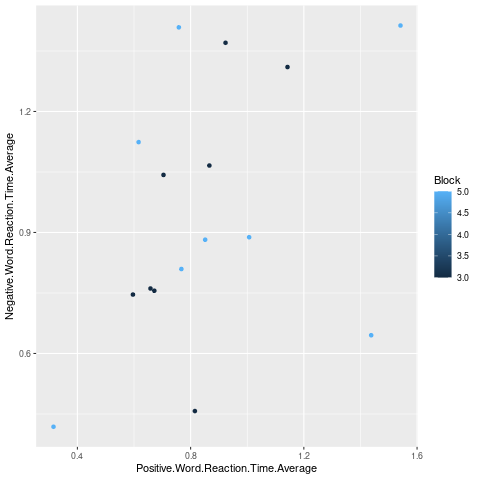
\includegraphics[width=.9\linewidth]{plot.png}
\end{center}

\section{Discussion}
\label{sec:org05d4142}


\addcontentsline{toc}{section}{References}
\bibliographystyle{apalike}
\bibliography{references}
\end{document}
